\documentclass[12pt,a4paper,oneside]{article}
\usepackage[colorlinks=true,unicode]{hyperref}
\usepackage[utf8]{inputenc}
\usepackage[czech]{babel}
\usepackage{graphicx}
\usepackage{pdfpages}
\usepackage{listings}             % Include the listings-package
\textwidth 16cm \textheight 25cm
\topmargin -1.3cm 
\oddsidemargin 0cm
\usepackage{footnote}
\pagestyle{empty}
\begin{document}
\title{Testování modulu ALTIMET01A}
\author{Jakub Kákona, Eva Pomíchalová;\\ kaklik@mlab.cz, evapomichal@gmail.com}
\maketitle

\thispagestyle{empty}
\begin{abstract}
\noindent
Při realizaci projektu ABL01A bylo zjištěno, že snímání tlaku z čidla MPL3115A2 funguje navzdory specifikaci výrobce minimálně do výšky 16 km což je cca 10 kPa. Na druhou stranu interní tlakový atmosférický model je použitelný pouze do výšky cca 10 km ve větších výškách vykazuje značné nepřesnosti. Cílem tohoto dokumentu je popsat přesnější měření a kalibrace čidla v případě použití v barometrickém výškoměru pro balonovou sondu ABL01A
\end{abstract}

\begin{figure} [htbp]
\begin{center}
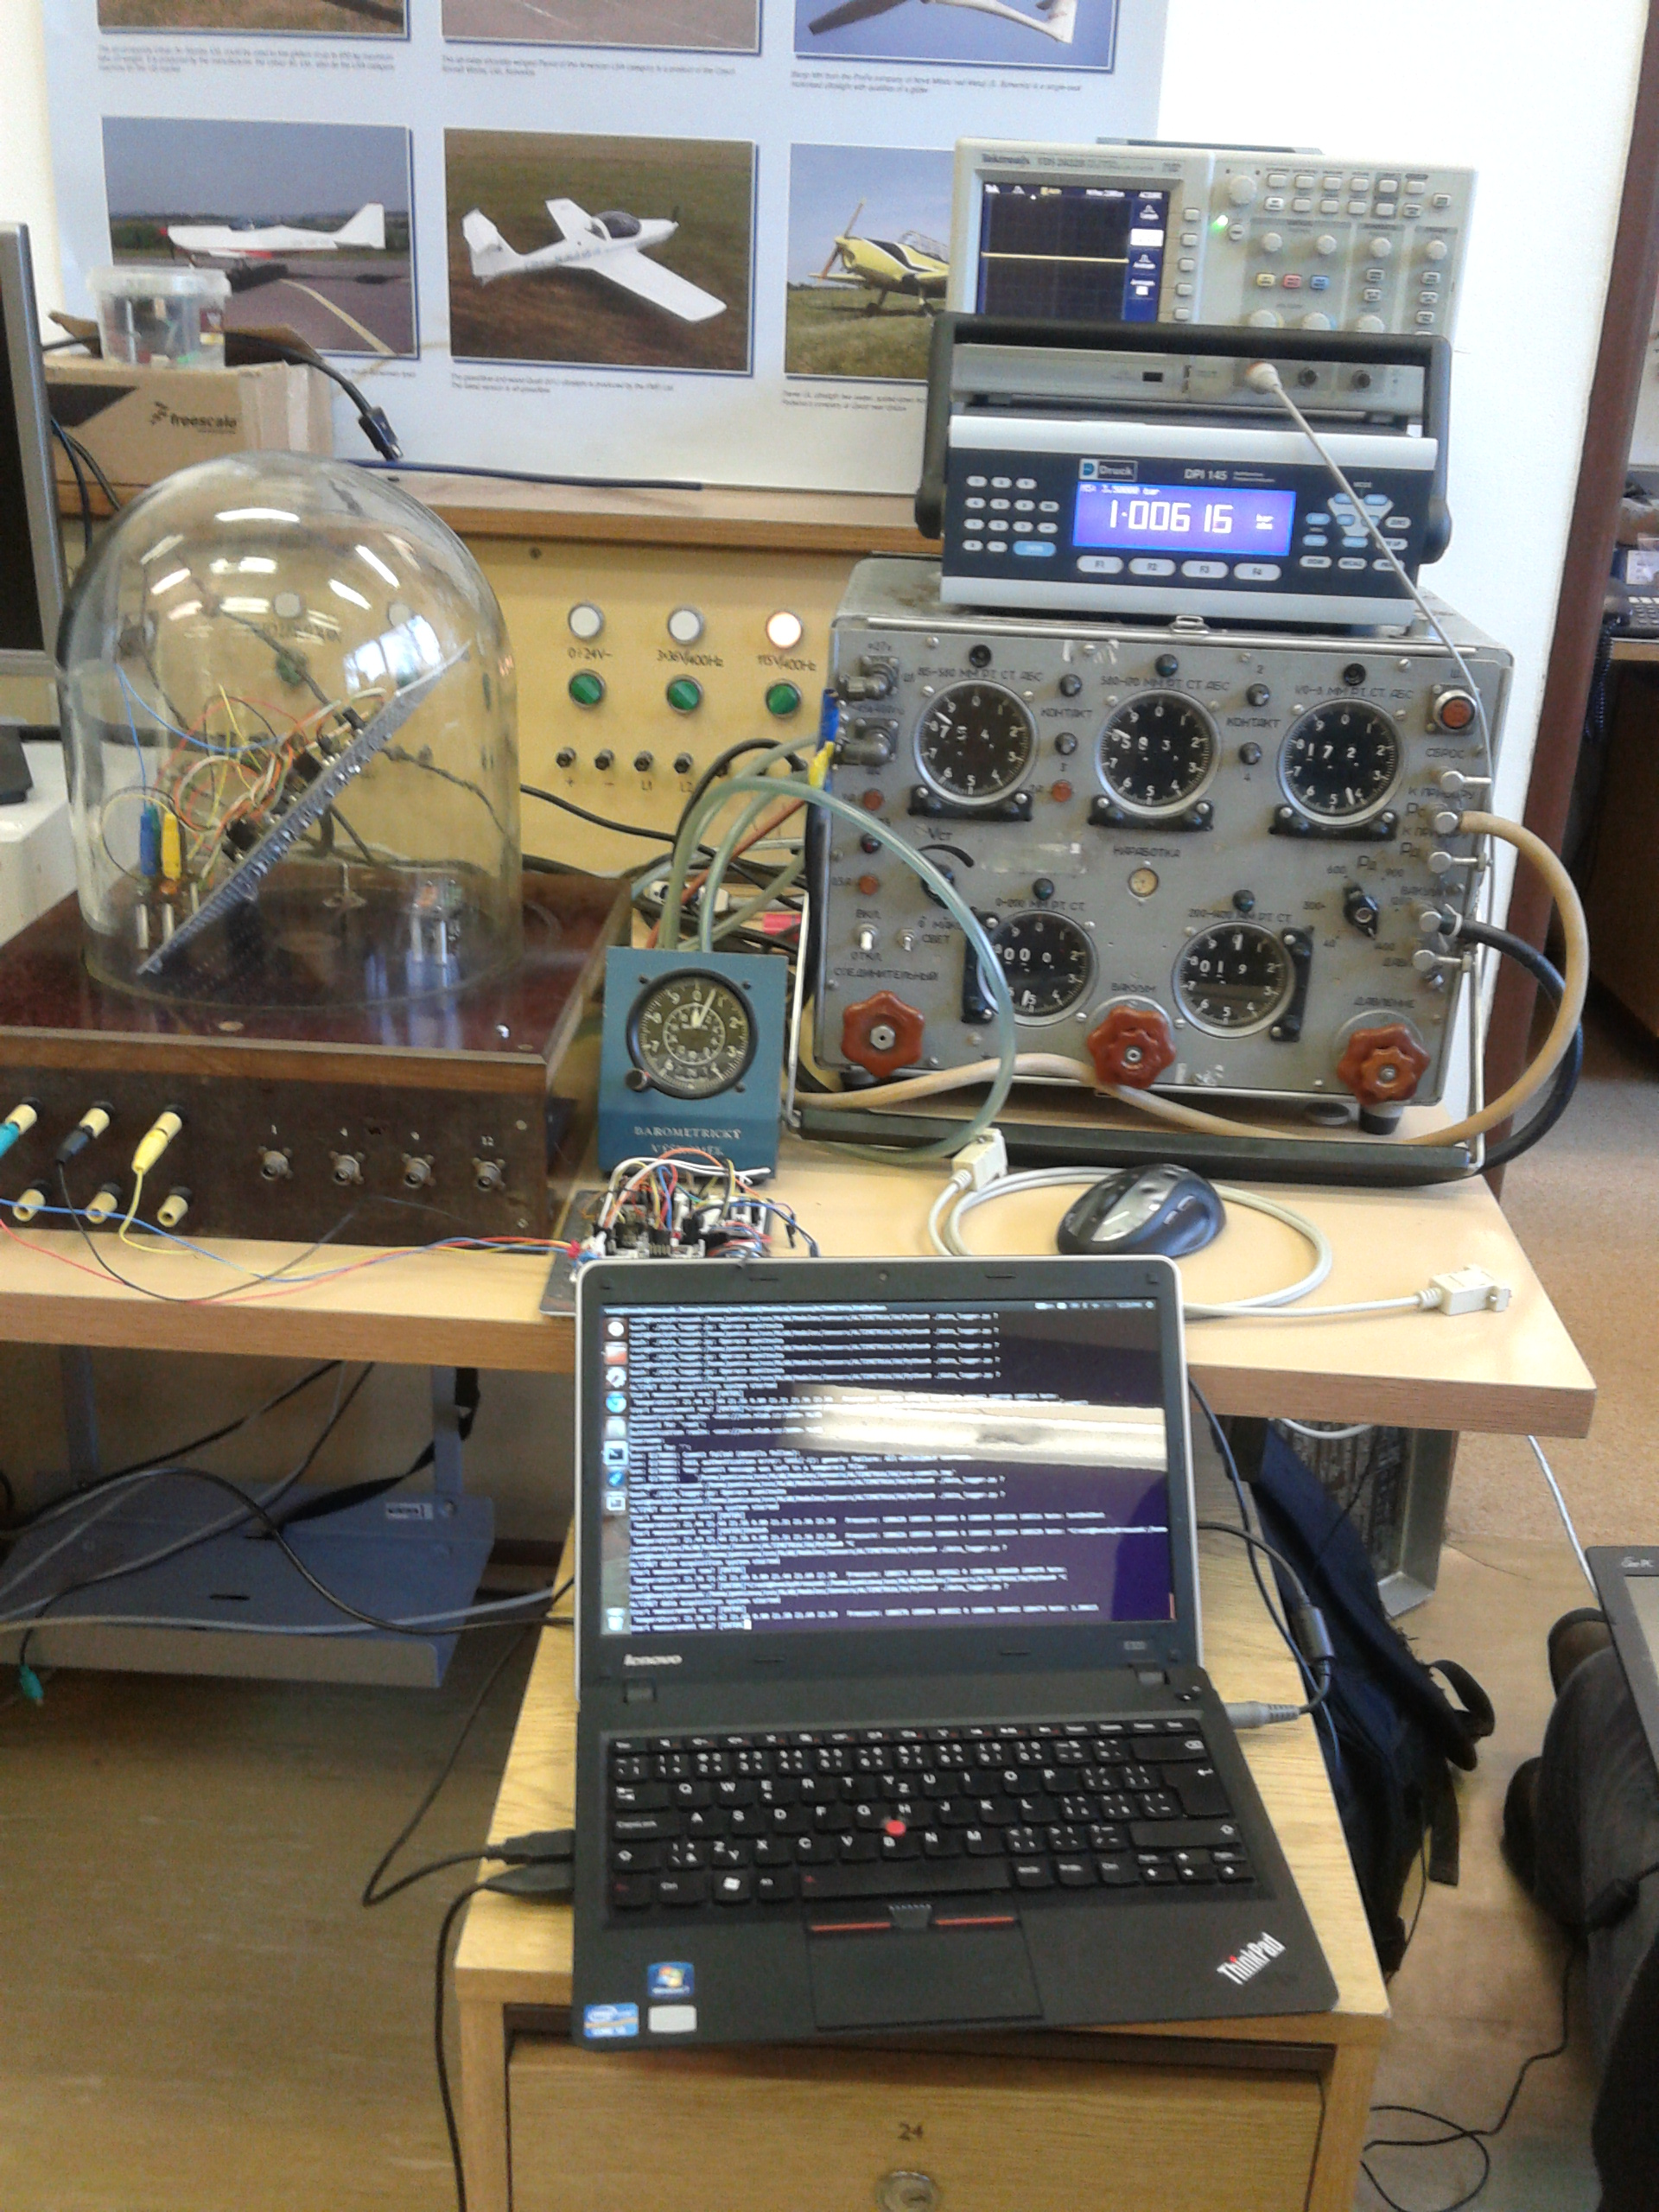
\includegraphics [width=80mm] {./img/altimet01a_testing_setup.jpg} 
\end{center}
\end{figure}

\begin{figure} [b]
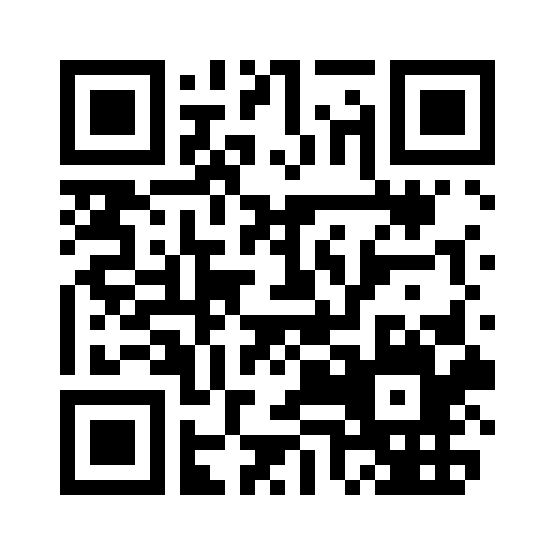
\includegraphics [width=25mm] {./img/ALTIMET01A_QRcode.png} 
\end{figure}

\newpage
\tableofcontents
\newpage

\section{Popis konstrukce}

Realizace testovacího systému pro čidlo MPL3115A2 využívá modulu I2CHUB02A, který umožňuje testování více čidel najednou. Čidla jsou tak společně umístěna ve vakuovém zvonu s řízeným tlakem a naměřené tlaky jsou společně s teplotami vyčítány I$^2$C sběrnici. Sběrnice I$^2$C byla z řídícího počítače vyvedena přes převodník i2c-avr-USB \cite{i2c_avr_USB}. 
Paralelně k hodnotám získaných z modulů ALTIMET je z řídícího počítače ještě vyčítán tlak měřený z referenčního měřícího přístroje DPI 145. 

Měřící přístroj DPI 145 byl do systému zapojen přes rozhraní RS232 za použití převodníku  RS232-USB. Nastavení komunikace je Parity=none, Speed=9600, Handshaking=none. (Způsob nastavení je možné nalézt v návodu k DPI145). 

\section{Programové vybavení}

Pro vyčítání čidel a záznam naměřených hodnot byl použit Python. Využívající speciálně vytvořenou knihovnu  \cite{MLAB-I2c-modules}. Tato knihovna řeší komunikaci se senzory MPL3115A2 v modulech ALTIMET01A. Samotný program je pak umístěn v dokumentační složce modulu ALTIMET01A \cite{data_logger}.

Na začánku programu je nadefinována topologie zapojení modulů, což je viditelné v následujícím bloku kódu (Odsazení bylo upraveno za účelem vložení na šířku stránky).

\lstset{language=Python}
\begin{lstlisting}[frame=single]
cfg = config.Config(
    port = port,
    bus = [
        {
            "type": "i2chub",
            "address": 0x72,
            
            "children": [
                {
                    "type": "i2chub",
                    "address": 0x70,
                    "channel": 3,
                    "children": [
{"name": "altimet1", "type": "altimet01" , "channel": 0, },   
{"name": "altimet2", "type": "altimet01" , "channel": 3, },   
{"name": "altimet3", "type": "altimet01" , "channel": 4, },   
{"name": "altimet4", "type": "altimet01" , "channel": 5, },   
{"name": "altimet5", "type": "altimet01" , "channel": 6, },   
{"name": "altimet6", "type": "altimet01" , "channel": 7, },   
                    ], 
                },
{"name": "altimet8", "type": "altimet01" , "channel": 6, },
            ],
        },
    ],
)
cfg.initialize()
\end{lstlisting}

Grafickou realizaci této topologie představuje obrázek \ref{test_setup_blocks}. V kterém jsou vynechána čísla portů na modulu I2CHUB02A. Podle nich jsou ve skutečnosti identifikována jednotlivá čidla, která jinak mají stejnou I2C adresu. Na sběrném počítači byl použit operační systém Linux Ubuntu 13.10.

\begin{figure} [htbp]
\centering
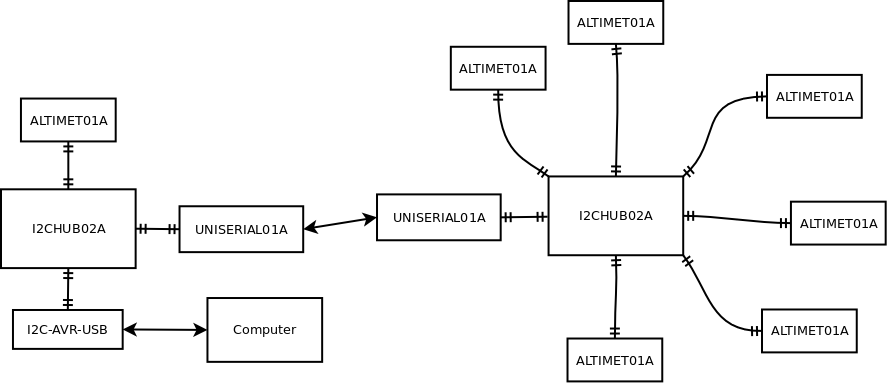
\includegraphics [width=220mm, angle=90, origin=c] {./img/test_setup.png}
\caption{Zapojení jednotlivých modulů v testovacím přípravku.}
\label{test_setup_blocks}
\end{figure}

\subsection{Čtení dat z přístroje DPI145}

Vzhledem k tomu, že přístroj byl připojený přes rozhraní RS232 a ke komunikaci používá protokol SCPI, tak bylo možné jej ovládat přímo z jazyka Python zápisem na seriové rozhraní počítače. V následujícím bloku je uveden testovací kód, který vyčte data zobrazena na displeji (Měřící přístroj musí být nastaven tak, aby na displeji byla přímo hodnota, kterou potřebujeme zaznamenat).

\begin{lstlisting}[frame=single]
#!/usr/bin/python

# Druck DPI 145  preassure measuring instrument test utility.  

import serial

ser = serial.Serial('/dev/ttyUSB0', 9600, timeout=1)
print ser.name
ser.write(':DISP?\n')
P_ref = eval(ser.readline(100))
sys.stdout.write("%s",P_ref)
ser.close()
\end{lstlisting}

Data jsou přijata ve formě stringu. Pro získání numerické proměnné by bylo třeba je parserovat  a vyhledávat číselný obsah. 

\section{Měření}

Blokové schéma měření je zobrazeno na obrázku \ref{test_block_scheme}.

\begin{figure} [htbp]
\centering
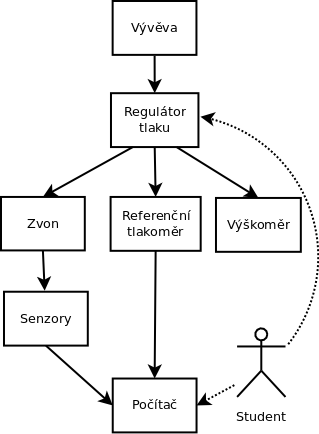
\includegraphics [width=100mm, origin=c] {./img/Diagram1.png}
\caption{Blokové schéma zapojení měření.}
\label{test_block_scheme}
\end{figure}

\subsection{Systém sběru dat z tlakových čidel}
Pro testování modulu ALTIMET01A s tlakovým čidlem MPL3115A2 byl vytvořen testovací přípravek využívající I2C a převodník i2c-avr-USB. Měřící systém byl ovládán skriptem napsaným v jazyce Python spouštěném na linuxovém počítači.  

\subsection{Výsledky}

Byly provedeny 3 měření z nichž použitelné byly 2 sady dat. V první sadě bylo použito pouze 5 senzorů, 1 byl nefunkční. V druhé sadě bylo stoupání ukončeno ve výšce přibližně 16 km z časových důvodů. Nicméně získaná data jsou pro účely práce dostačující.

Na obrázku \ref{KorekceTlaku} je porovnání údajů ze senzorů oproti údajům z DPI 145. Naměřené hodnoty byly proloženy přímkou. Hodnoty koeficientů pro jednotlivé senzory jsou následující.

\newpage

\begin{verbatim}
Final set of parameters            Asymptotic Standard Error
=======================            ==========================

k1              = 0.998531         +/- 0.0004952    (0.04959%)
q1              = 1.00027          +/- 25.23        (2522%)

k2              = 0.999998         +/- 0.0005202    (0.05202%)
q2              = 1                +/- 26.47        (2646%)

k3              = 0.998286         +/- 0.0002962    (0.02967%)
q3              = 171.628          +/- 15.05        (8.77%)

k4              = 0.999579         +/- 0.001141     (0.1142%)
q4              = 1.00012          +/- 58.07        (5807%

k5              = 1.00002          +/- 0.0002655    (0.02655%)
q5              = 84.5852          +/- 13.49        (15.95%)

k6              = 1.00217          +/- 1.274e+10    (1.271e+12%)
q6              = 1.00217          +/- 1.274e+10    (1.271e+12%)
\end{verbatim}

Při bližším zkoumání grafu v části s nízkými hodnotami tlaku \ref{KorekceTlakuZoom}, lze nalézt drobné odchylky hodnot od aproximace přímkou. Pokud by tyto odchylky byly několikanásobně větší, znamenalo by to, že senzory neměří přesně oproti DPI145. Odchylky jsou však jen drobné, proto lze usuzovat, že senzory měří i ve vyšších výškách než udává výrobce minimálně s takovou přesností jako DPI145.

Pro rozšíření informací o přístrojích používaných v laboratoři se lze podívat na obrázek \ref{stoupani}, na kterém vidíme rychlost "stoupání" do výšky téměř 19 km. Stoupání bylo simulováno vývěvou, která odsávala vzduch z vakuového zvonu, ve kterém byly uloženy senzory. Tlak vzduchu byl regulován ručně studentem provádějícím měření přes regulátor, který je zachycen na obrázku na úvodní stránce zprávy.

Výška byla vypočítána pomocí barometrické rovnice. Pro zajímavost lze porovnat zobrazení závislosti tlaku a výšky vypočítané pomocí barometrické rovnice z naměřených "kalibrovaných" hodnot \ref{tlak_vyska} a stejnou závislost v grafu pro mezinárodní standardní atmosféru \ref{MSA}. 

\begin{figure} [htbp]
\centering
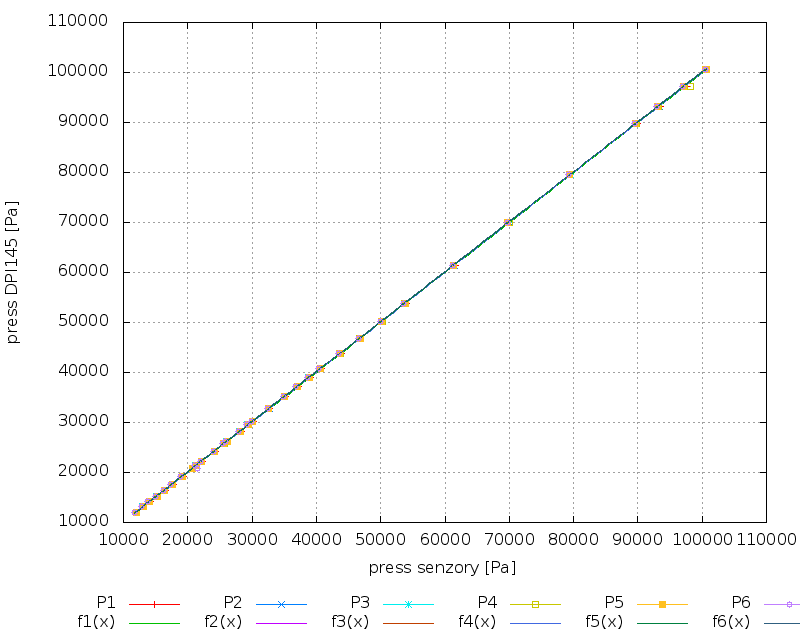
\includegraphics [width=130mm, origin=c] {./img/KorekceTlaku.png}
\caption{Senzory vs. DPI145.}
\label{KorekceTlaku}
\end{figure}

\begin{figure} [htbp]
\centering
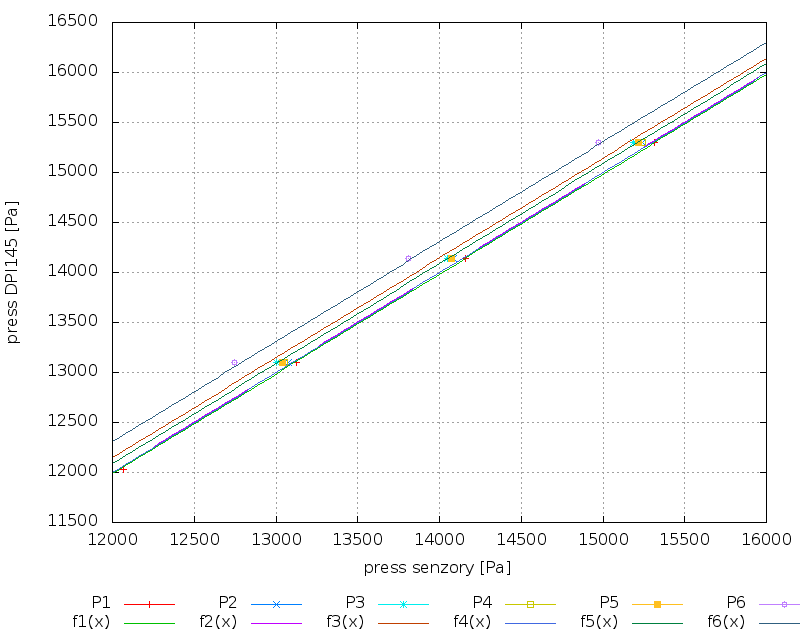
\includegraphics [width=130mm, origin=c] {./img/KorekceTlakuZoom.png}
\caption{Hodnoty proložené přímkou - detail pro nízké hodnoty tlaku.}
\label{KorekceTlakuZoom}
\end{figure}

\begin{figure} [htbp]
\centering
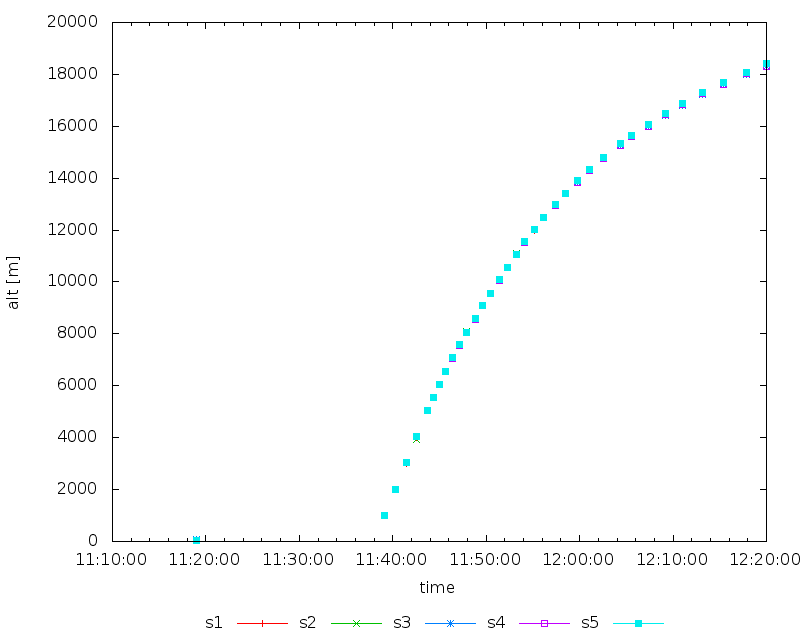
\includegraphics [width=130mm, origin=c] {./img/Stoupani.png}
\caption{Stoupání.}
\label{stoupani}
\end{figure}

\begin{figure} [htbp]
\centering
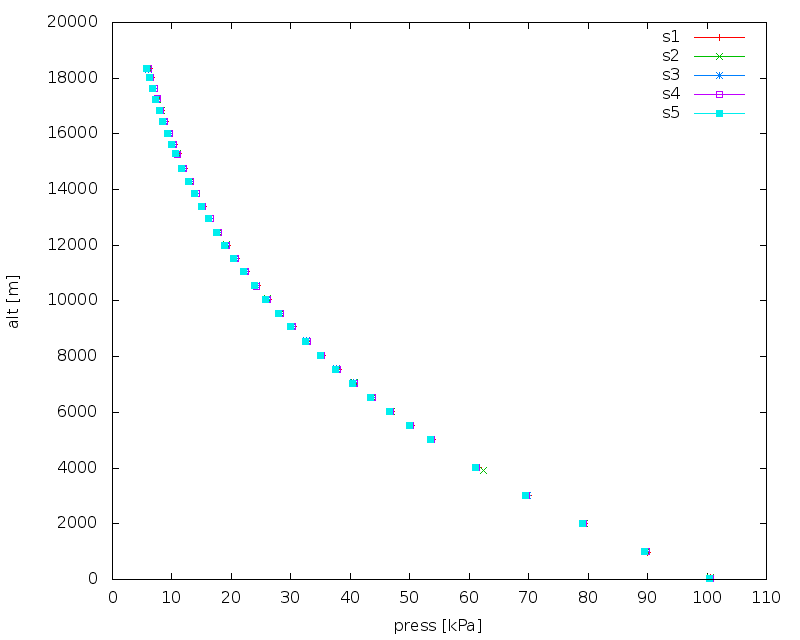
\includegraphics [width=130mm, origin=c] {./img/Tlak_vyska.png}
\caption{Tlak vs. výška.}
\label{tlak_vyska}
\end{figure}

\begin{figure} [htbp]
\centering
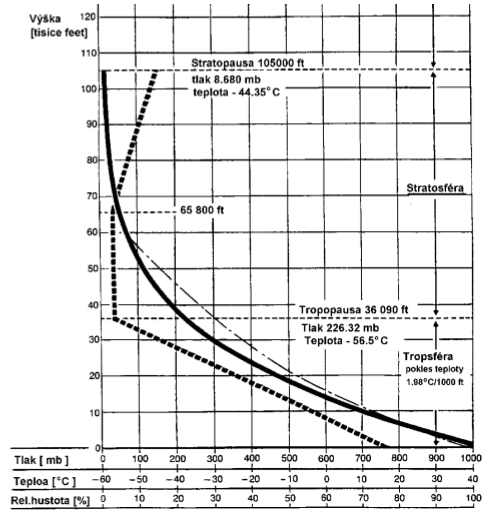
\includegraphics [width=100mm, origin=c] {./img/graf.png}
\caption{Mezinárodní standardní atmosféra.}
\label{MSA}
\end{figure}

\subsection{Nejistota}
Nejistotu lze spočítat podle následujících vzorců. Byla spočítaná tzv. rozšířená nejistota. Vzorec platí za předpokladu, že chyby jsou rovnoměrně rozložené.
$u_{DPI}$ označuje nejistotu tlakoměru DPI145, $u_s$ označuje nejistotu senzorů udávanou výrobcem v rozsahu 70-110 kPa. $u_{st}$ je potom tzv. standardní nejistota a $u_{aug}$ nejistota rošířená.

\begin{equation}
u_{DPI} = 0.0002 \cdot rdg + 0.0001 \cdot FS
\end{equation}
\begin{equation}
u_{s} = 0.005 kPa
\end{equation}
\begin{equation}
u_{st} = \sqrt{u_{DPI}^{2}+u_{s}^{2}}
\end{equation}
\begin{equation}
u_{aug} = \frac{2}{\sqrt{3}} \cdot u_{st}
\end{equation}

Například pro naměřenou hodnotu tlaku 0.30259 kPa vyjde nejistota 0.30669 kPa. Tato chyba je oproti chybě senzorů udávané výrobcem velmi vysoká. Proto není možné senzory pomocí přístroje DPI145 kalibrovat. Přesnost DPI145 by bylo vhodné vylepšit vhodnějším nastavením rozsahu, to by ovšem zmenšilo chybu pouze 2.6x což stále není přesnější než senzory.

\subsection{Závěr}

\begin{itemize}
\item Nebyl nastaven optimálně měřící rozsah přístroje DPI145. Z hlediska nejistoty by bylo vhodnější nastavit menší rozsah.
\item Použité přístroje nevykázaly žádné potíže ani ve výškách vyšších než 11 km. Pouze vakuování zvonu ve vyšších výškách trvalo delší dobu.
\item Senzory měří i mimo výrobcem udávaný rozsah (ve větších výškách) a to minimálně se stejnou přesností jako přístroj DPI145.
\item Senzory jsou v rozsahu udávaném výrobcem dle jejich katalogového listu přesnější než přístroj DPI145.
\item Senzory není možné kalibrovat pomocí přístroje DPI145.
\item Naměřené hodnoty přibližně odpovídají hodnotám MSA. Do cca 18 km nejsou vykázány žádné výrazné změny oproti MSA, ačkoli obecně barometrická rovnice platí pouze do 11 km. Pro účely tohoto měření a zobrazení postačí.
\end{itemize}



\begin{thebibliography}{99}
\bibitem{MLAB-I2c-modules}{https://github.com/MLAB-project/MLAB-I2c-modules} 
\href{https://github.com/MLAB-project/MLAB-I2c-modules}{MLAB-I2c-modules}
\bibitem{data_logger}{svn://svn.mlab.cz/mlab/Modules/Sensors/ALTIMET01A/SW/Python} 
\href{svn://svn.mlab.cz/mlab/Modules/Sensors/ALTIMET01A/SW/Python}{MLAB-I2c-modules}
\bibitem{i2c_avr_USB}{http://wiki.mlab.cz/doku.php?id=cs:i2c\_avr\_usb} 
\href{http://wiki.mlab.cz/doku.php?id=cs:i2c_avr_usb}{i2c-avr-USB}
\end{thebibliography}
\end{document}